\def\year{2020}\relax

\documentclass[letterpaper]{article} %DO NOT CHANGE THIS
\usepackage{aaai20}  %Required
\usepackage{times}  %Required
\usepackage{helvet}  %Required
\usepackage{courier}  %Required
\usepackage{url}  %Required
\usepackage{graphicx}  %Required
\frenchspacing  %Required
\setlength{\pdfpagewidth}{8.5in}  %Required
\setlength{\pdfpageheight}{11in}  %Required
\setcounter{secnumdepth}{0}  
\usepackage{subfigure}

\begin{document}
% The file aaai.sty is the style file for AAAI Press 
% proceedings, working notes, and technical reports.
%
\title{A Genetic Approach to the Formulation of Tetris Engine}
\author{Jiachen Zhang, Miaoqi Zhang, Shuheng Cao\\
\{j756zhan, m337zhan, s53cao\}@uwaterloo.ca\\
University of Waterloo\\
Waterloo, ON, Canada\\
}
\maketitle

%%%%%%%%%. Abstract %%%%%%%%%

\begin{abstract}
{\bf Complete this section for D4.}

The {\it Abstract} should be at most 150 words long, and should summarize briefly what your project is about.  This includes the motivation for the problem (2-3 sentences), the problem you tackled (2-3 sentences), and your main results (1-2 sentences).   
\end{abstract}

%%%%%%%%%. Introduction %%%%%%%%%

\section{Introduction} 

% The {\it Introduction} section ($\sim$1 page) describes the background and motivation behind your work, and provides an overview of the work and the findings.  It should include the following content.  
%
\begin{itemize} 

\item 
{\bf Motivations}
% {\bf Complete this part for D1.}

% Motivate your entire paper.  At a high level, describe the problem that your project is addressing.  Why is this an important problem to tackle?  If there a solution to this problem, what are some potential real-world impacts of this solution?  Try to give a compelling motivating story.  If possible, support your argument with evidence such as facts and statistics.  (2-3 paragraphs)

With the great triumph of AlphaGo in 2016, more and more researchers are interested in using machine learning techniques to solve more advanced and complicated games such as StarCraft II. However, in the authors' opinion, it also provides us an invaluable opportunity to revisit some of the traditional video games, aiming for more reliable and satisfying results. Consequently, this project's primary motivation is to introduce, implement, and compare several different approaches to tackle the Tetris, a tile-matching video game with enduring appeal and popularity. A more detailed introduction and instruction of Tetris will be presented in the {\it Methodology} section since the authors implemented a Tetris in Python for visualization and illustration purpose.

Solving Tetris is a crucial and intriguing topic due to the two reasons below. On the one hand, Tetris is essentially an extraordinary optimization problem because each game will end no matter how well they are placed \cite{burgiel_1997}, so there is no such thing as perfect solutions to Tetris and there is always room to improve. On the other hand, the analyses and comparisons mentioned in this report are not limited to Tetris only, where we could broaden them to real-life problems, such as self-driving cars and robotics, with ease.

Finally, as mentioned in the {\it Discussion} section, one of the main problems the machine learning community faces is the lack of explainability and interpretability for most of the models. The direct analyses on most of the recent models, such as AlphaGo and AlphaZero, are notoriously complicated and challenging, but with a more straightforward and simplified setup like Tetris, it gives us more opportunities to have a more in-depth insight into what is happening under the hood. Consequently, the results from simple setups will contribute to a better and deeper understanding of the more complex models.

\item 
{\bf Methodologies}
% {\bf For D1, describe the problem and your methodologies only.  Then, complete this part for D4. }

% Describe, at a high-level, the problem you tackled and your main results.  What research questions are you trying to answer?   What methodologies did you used to answer the question? What are the performance measures that you used to evaluate the methodologies?   Describe your key findings in 2-3 sentences. (2-3 paragraphs)
In brief, the methodology of this project consists of four main parts, as shown below.
\begin{itemize}
  \item 
  First and foremost, we built a Tetris interface for both visualization and training purposes. For the sake of communication with our models, the interface is written in Python. 
  \item 
  Next, we solved the problem using a hand-crafted agent, where we manually chose the weights for 4 most representative state features, the number of holes, the height of the highest column, the height of each column, and the difference in height between consecutive columns \cite{Bertsekas_1996}. This approach is based mainly on the heuristic search algorithm and involves a lot of trails-and-errors. The result serves as the benchmark for the project.
  \item 
  On top of that, we also tackled the problem from an AI engineer's perspective. The main idea is to use a genetic algorithm to automatically find an optimal weight combination for 9 state features, where the detailed description for the features could be found in the Methodology section.  After 200 training epochs, we indeed get a result surpassed the benchmark.
  \item 
  Ultimately, we added more functionalities to the traditional Tetris, like introduce the ability to see the next Tetromino and enable holding the unwanted Tetromino, and the retrained model yields satisfying results, which proved the ability to generalization.
\end{itemize}


\item 
{\bf Complete this bullet point for D4.}

Emphasize your contributions.  How should we interpret the results?  Why should people care about this work?   Does this project introduce any novel techniques or reveal any unexpected findings?  In bullet point forms, list 3-4 key contributions of your project.

\end{itemize}

%%%%%%%%%. Related Work %%%%%%%%%

\section{Related Work} 

{\bf Complete this section for D1.}

The {\it Related Work} section ($\sim$1 page) summarizes prior work for addressing the same problem or similar problems.  
%
In this section, you should aim to survey at least 5-7 papers. Whenever possible, synthesize the literature by describing multiple papers in aggregate, i.e., mentioning a common technique that multiple prior work used.  Try to connect the prior work into a coherent story.  Imagine that you are describing a story to someone about how researchers have used different techniques over time to solve the same or similar problems.  Please use BibTeX to do citations.  Here are some examples \cite{SS14,Block62,Novikoff62}.


%%%%%%%%%. Methodology %%%%%%%%%

\section{Methodology}

{\bf Complete this section for D2.}

The {\it Methodology } section ($\sim$2 pages) describes the algorithms that you chose to implement.  Describe in details how each algorithm works.  Include their mathematical formulations, if necessary.  Include pseudo-code, if necessary.  If you had to extend an existing algorithm in order for it to work with the problem, describe in details what is different/new.  Provide a rationale for why you selected these particular algorithms and how they are appropriate for the problem.  You should provide enough details so that someone can reproduce the steps and replicate your results.  

If you are tackling a machine learning problem, you may be using an existing data set or creating a new data set.  In this case, you should describe the data-set that you are analyzing as well as any data filtering and merging procedures that you used to prepare/create your data-set.  Your description should. include the size of the data-set(s) (i.e., number of examples), whether the class labels are balanced/imbalanced, the meaning of the features, and other unique characteristics of the data-sets.   Explain why the data-sets are appropriate for your problem and what are their limitations.  Include the URL of the websites from which you downloaded the data-set(s).

You should also describe any pre-processing steps you took to prepare or create the final data-set that you used to train and test the algorithms.  Examples of pre-processing steps include procedures for joining multiple data-sets, filtering out certain examples, scaling features, etc.  Provide the rationale for why you are using these data preparation procedures, with enough details so that someone can reproduce the steps and replicate your results.   For example, if you chose to re-scale certain features, explain how the re-scaling was done and why.   


%%%%%%%%%. Example of subfigure and 2-column figure layout %%%%%%%%%

\begin{figure*}[t!]
\centering
\subfigure[image A]{
\fbox{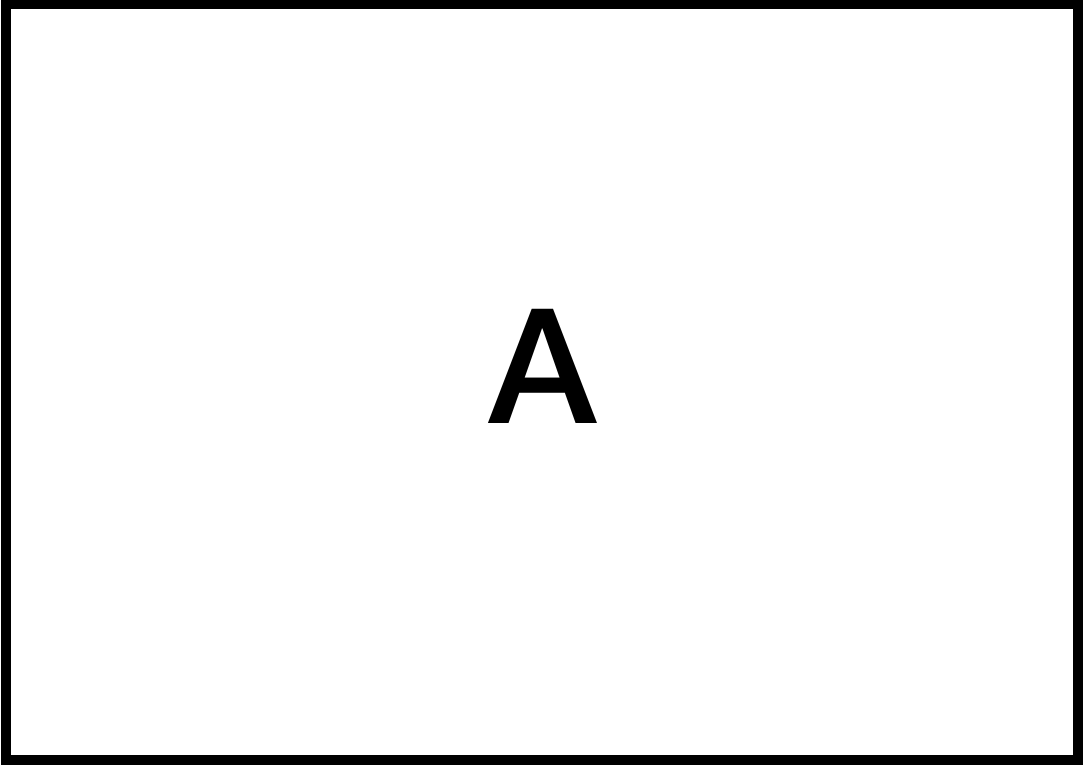
\includegraphics[height=2.6cm]{figures/A}}
\label{fig:a}
}\hfill
\subfigure[image B]{
\fbox{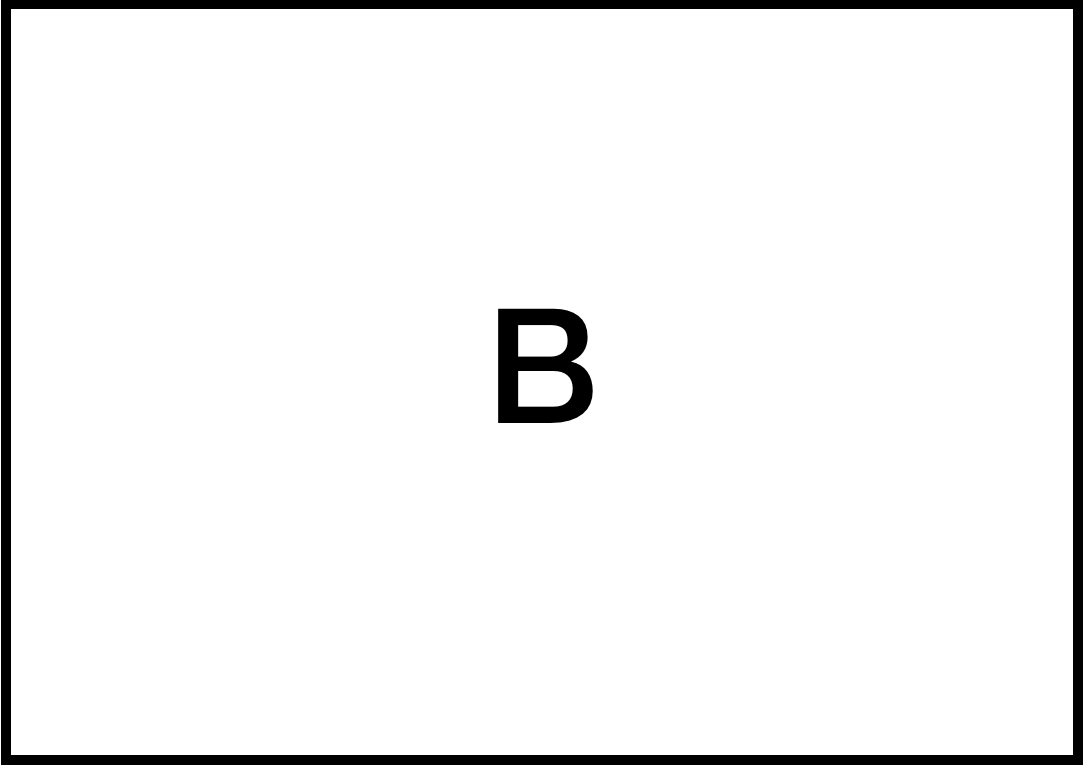
\includegraphics[height=2.6cm]{figures/B}}
\label{fig:b}
}\hfill
\subfigure[image C]{
\fbox{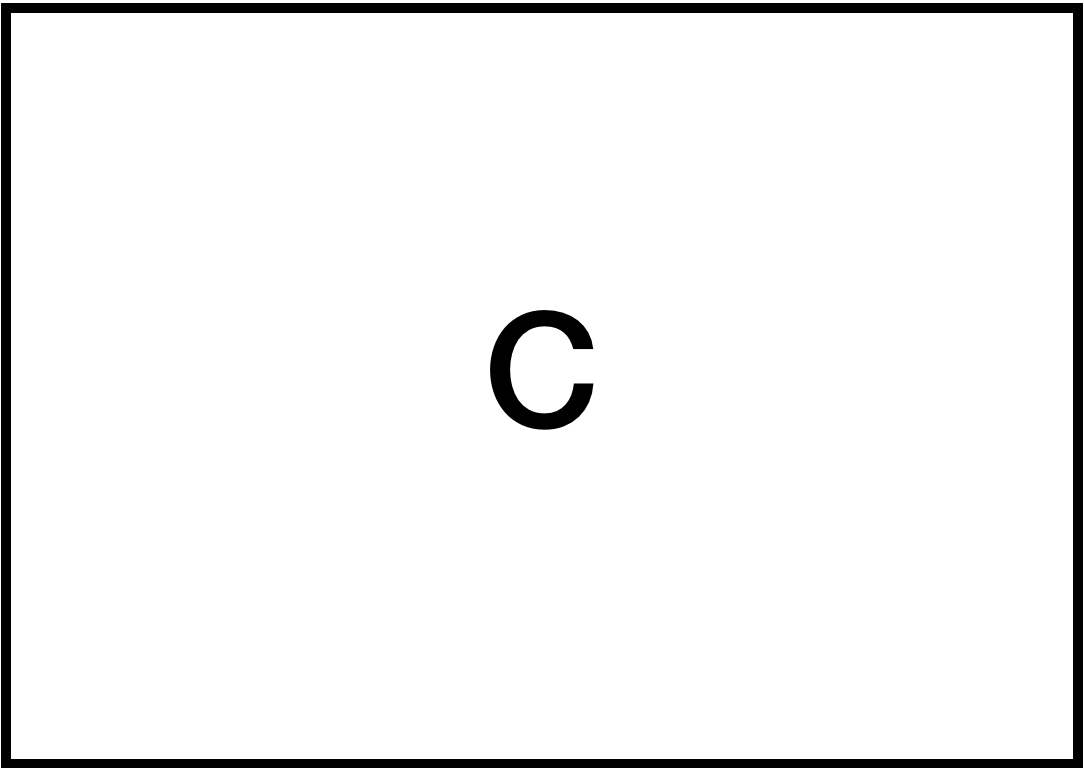
\includegraphics[height=2.6cm]{figures/C}}
\label{fig:c}
}\hfill
\subfigure[image D]{
\fbox{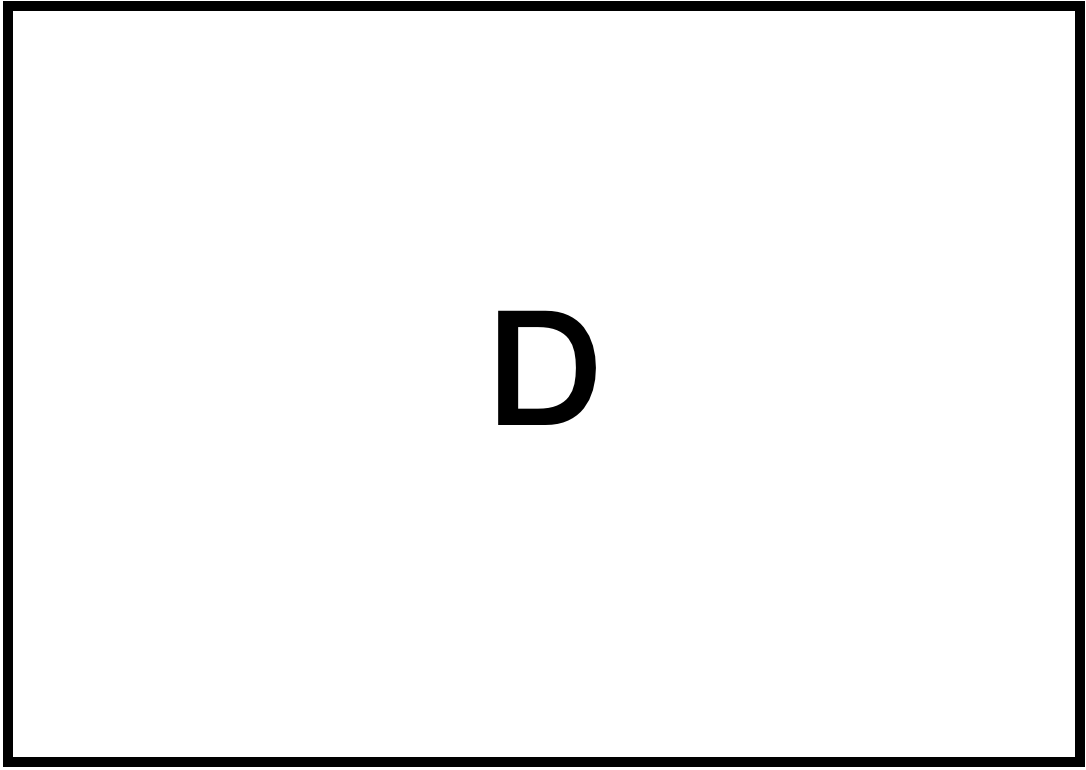
\includegraphics[height=2.6cm]{figures/D}}
\label{fig:d}
}\hfill
\caption{Another example of figure layout}
\label{fig:figures_across}
\end{figure*}

%%%%%%%%%. Results %%%%%%%%%

\section{Results}

{\bf Complete this section for D2 and D3.}

The {\it Results} section ($\sim$2 pages) describes how you evaluated the algorithms and reports the findings.  

{\bf Complete the following two paragraphs for D2.}

Describe the measures that you used to evaluate the algorithms.  Be as precise as possible by including their mathematical formulations.  Provide a rationale for why these performance metrics are appropriate for your problem.

Describe other details about your experimental design.  If you are tackling a machine learning problem, include details such as how you created the training, validation and test set, how you selected the model's hyper-parameters, etc.    

{\bf Complete the following two paragraphs for D3.}

Describe the findings from your evaluation.  Describe both (a) how well your techniques worked, and (b) what you learned about the problem through these techniques.  

Prepare figures (e.g., Figure \ref{fig:results2}) and tables (e.g., Table \ref{tab:results1}) to describe your results clearly.  Make sure to label your figures and tables and explain them in the text.  If you are comparing the performance of algorithms, include statistical tests to assess whether the differences are statistically significant.  If possible, describe how your techniques compare to prior work.  

\begin{table}[h!]
    \centering
    \normalsize{
    \begin{tabular}{ l c }
    \hline
         Techniques & F-1 Score\\
         \hline
          Baseline & 0.80 \\
          Another Baseline & 0.76\\
          My Awesome Algorithm & {\bf 0.95}\\
         \hline
    \end{tabular}}
    \caption{example of a table summarizing the results}
    \label{tab:results1}
\end{table} 

\begin{figure}[htbp!]
  \centering
  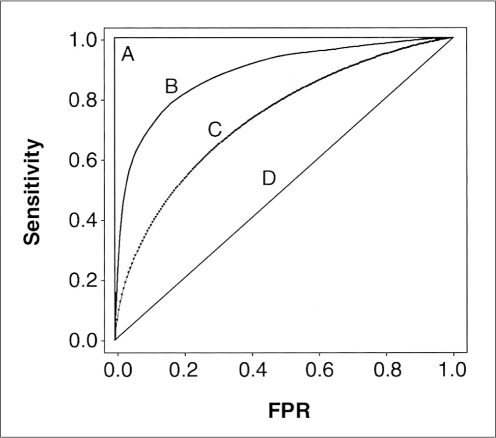
\includegraphics[width=0.9\linewidth]{figures/roc.png}
  \caption{ROC curve of my awesome algorithms}
  \label{fig:results2}
\end{figure}


%%%%%%%%%. Discussion %%%%%%%%%

\section{Discussion}

{\bf Complete this section for D4.}

The {\it Discussion} section ($\sim$1 pages) describes (a) the implications of your results, and (b) the impact and the limitations of your approach.  

For the results, describe how a reader should interpret them.  Try to form concise take-away messages for the reader.  For your approach, describe the extent to which your approach helps to solve the problem.  Describe any limitations of your approach.  If possible, compare your results and your approach to that of prior work. 

%%%%%%%%%. Conclusion %%%%%%%%%

\section{Conclusion}

{\bf Complete this section for D4.}

The {\it Conclusion} section ($\sim$0.5 pages) provides a brief summary of the entire paper.  In this section, describe 
\begin{itemize}
    \item the motivation, the problem, and your results, and
    \item 3-4 promising future directions.
\end{itemize}

%%%%%%%%% Bibliography %%%%%%%%%
\newpage
\bibliographystyle{aaai}
\bibliography{report}

\end{document}
